\tdplotsetmaincoords{60}{110}

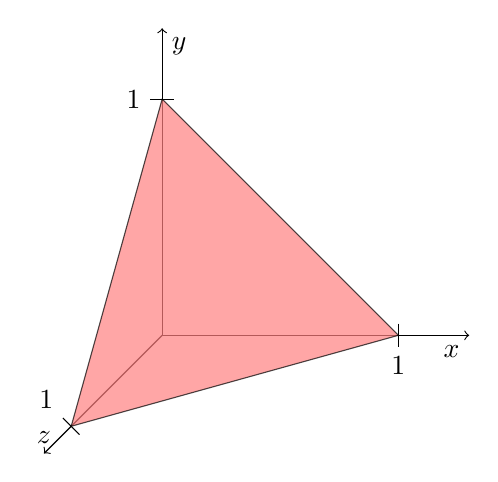
\begin{tikzpicture}[scale=3]
    \begin{scope}
        \draw[->] (0,0,0) -- (1.3,0,0) node[anchor=north east]{$x$};
        \draw[->] (0,0,0) -- (0,1.3,0) node[anchor=north west]{$y$};
        \draw[->] (0,0,0) -- (0,0,1.3) node[anchor=south]{$z$};
        \draw [fill=red!50, opacity=0.7] (0,0,1)--(1,0,0)--(0,1,0)--cycle;
        \draw (1,0.05,0) -- (1,-0.05,0) node[anchor=north]{$1$};
        \draw (0.05,1,0) -- (-0.05,1,0) node[anchor=east] {$1$};
        \draw (0.035,-0.035,1) -- (-0.035,0.035,1) node[anchor=south east]{$1$};
        
    \end{scope}
\end{tikzpicture}

%%% Local Variables: 
%%% mode: latex
%%% TeX-master: "../../main"
%%% End: 
